%==========================================================
%-------------------- begin preamble ----------------------
%==========================================================
%\documentclass[12pt]{article}
\documentclass[12pt, a4paper, abstracton]{scrartcl}
\setkomafont{disposition}{\normalfont\bfseries}
\usepackage{Setup/style}
%---------------- custom style -----------------------
%----- equation numbering -------
\numberwithin{equation}{section}     % number within section
%\numberwithin{equation}{subsection} % number within subsection

%----- fig & table numbering -----
\counterwithin{figure}{section}
\counterwithin{table}{section}

%--------- format abstract ---------
\makeatletter
\renewenvironment{abstract}{
    \if@twocolumn
      \section*{\abstractname}
    \else
      \begin{center}
        {\bfseries \large\abstractname\vspace{\z@}}
      \end{center}
      \quotation
    \fi}
    {\if@twocolumn\else\endquotation\fi}
\makeatother

%----------------- tikz ---------------------------
% Define block styles
\tikzstyle{startstop} = [rectangle, rounded corners,
    minimum width=3cm, minimum height=1cm,text centered, draw=black, fill=red!30]
\tikzstyle{io} = [trapezium, trapezium left angle=70, 
    trapezium right angle=110, minimum width=3cm, minimum height=1cm, text centered, text width=3cm, draw=black, fill=blue!30]
\tikzstyle{process} = [rectangle, minimum width=3cm,
    minimum height=1cm, text centered, text width=3cm, 
    draw=black, fill=orange!30] 
\tikzstyle{decision} = [diamond, minimum width=3cm, 
    minimum height=1cm, text centered,text width=2cm, 
    draw=black, fill=green!30]
\tikzstyle{arrow} = [thick,->,>=stealth]
\tikzstyle{block} = [rectangle, draw, fill=blue!20, 
    text width=5em, text centered, rounded corners, minimum height=4em]
\tikzstyle{line} = [draw, -latex']
\tikzstyle{cloud} = [draw, ellipse,fill=red!20, node distance=3cm,
    minimum height=2em]


%---------- insert custom LaTeX commands ----------
\newcommand*{\QED}{\hfill\ensuremath{\square}}
\newcommand{\E}{\mathrm{E}}
\newcommand{\R}{\mathbb{R}}
\newcommand{\X}{\mathbf{X}}
\newcommand{\y}{\mathbf{y}}
\newcommand{\rss}{\mathrm{RSS}}
\newcommand{\MSE}{\mathrm{MSE}}
\newcommand{\Err}{\mathrm{Err}}
\newcommand{\err}{\mathrm{err}}
\newcommand{\bias}{\mathrm{Bias}}
\newcommand{\Var}{\mathrm{Var}}
\DeclareMathOperator*{\argmax}{arg\,max}
\DeclareMathOperator*{\argmin}{arg\,min}
\DeclareMathOperator*{\cv}{CV}
\DeclareMathOperator*{\df}{df}
\newcommand{\T}{\mathcal{T}}

\NewDocumentCommand{\cw}{v}{%
\textbf{\texttt{\textcolor{Blue}{#1}}}%
}


\addbibresource{bibliography.bib}   % Bibliography

% Set graphics path
\graphicspath{{latex/figures/}}

%-------- header & foot -------- 
% FILL IN APPROPRIATE DESCRIPTIONS
% title page
\pagestyle{fancy}
\fancypagestyle{firststyle}
{
   \fancyhf{}
   \fancyfoot[C]{
   % Link to GitHub
   \faGithub \ 
   \href{https://github.com/nicolossus}{github.com/nicolossus}}
   \renewcommand{\headrulewidth}{0pt}
   \renewcommand{\footrulewidth}{0.4pt}
}
% rest of document
\fancyhead[L]{\small FYS4411}       % Set <course>
\fancyhead[C]{\small Project 2}             % Set <title>    
\fancyhead[R]{\small June 1, 2022}   % Set <date>
\fancyfoot[C]{-- \thepage\ --}
\renewcommand{\headrulewidth}{0.4pt}
\renewcommand{\footrulewidth}{0.4pt}
%==========================================================
%-------------------- end preamble ----------------------
%==========================================================

%==========================================================
%-------------------- main content ----------------------
%==========================================================
\begin{document}
%------------------ title -------------------------
%================================================================
%------------------------ Title Page ----------------------------
%================================================================
\newcommand{\horrule}[1]{\rule{\linewidth}{#1}} %Horizontal rule
\titlehead{
\includegraphics[scale=0.35]{latex/latex-report/Images/Logo/UiO/UiO_Seal_A_ENG.pdf}}
\title{
\large \textsc{Course code: Course name} % Set <COURSE>
\\ [25pt]
\horrule{0.5pt} \\[0.4cm]
\huge TITLE}               % Set <TITLE>
\subtitle{SUBTITLE         % Set <SUBTITLE>
\horrule{2pt} \\[0.5cm]}
\author{AUTHOR}            % Set <AUTHOR>, separate multiple                                 % authors with \and
\date{Month Day, Year}     % Set <DATE>

\maketitle

\pagenumbering{gobble}
\thispagestyle{firststyle}

%---------------- abstract -------------------------
%================================================================
%------------------------- Abstract -----------------------------
%================================================================
\begin{abstract}
The many-body wave function increases exponentially in complexity with the number of particles, and therefore, clever approximations to it is of great interest. The universal approximation theorem states that any function can be approximated to an arbitrary error by a neural network. We will therefore seek to implement an approach based on a machine learning method. 
An approach based on a neural network for solving the quantum mechanical wave function is still a relatively new, but an increasingly interesting prospect \citep{Saito_2018}. 
This project analyzes two systems of electrons, a quantum dot in a one-dimensional harmonic oscillator trap and a pair of interacting electrons in an isotropic two-dimensional harmonic oscillator trap. We analyze the systems using an unsupervised learning method, the restricted Boltzmann machine (RBM), to simulate the wave function (known as a Neural-network Quantum State\citep{Carleo_2017}), and generate upper bound estimates to the ground state energies using two Markov Chain Monte Carlo algorithms. We perform some coarse searches in the space of hyper parameters, like learning rate, batch-sizes for optimization and number of neurons in hidden layer. After finding the optimal set of parameters, we find that we approximate the ground state energy for the quantum dot in a single dimension to a high degree of precision. We find the best approximation to the ground state energy to be $E_0 = 0.499999 \pm 3\cdot10^{-6}$ a.u, using the RWM sampling algorithm. For the system of two interacting electrons in two-dimensional space we find the best approximation, again via the RWM sampling algorithm, to be $E_0 = 3.059 \pm 0.008$ a.u. Knowing the true ground state energy to be $E_0=3.0$ a.u \citep{PhysRevA.48.3561}, there is still plenty of room for improvement.
\end{abstract}   % Abstract on title page
\newpage

%------------ content overview ---------------------
\frontmatter      % Folios in Roman numerals
\tableofcontents    
%\abstractintoc   % Add abstract to table of contents
%\listoffigures      
%\listoftables       
%\listofalgorithms
%\listoftodos       % list TODOs

%----------------- body ----------------------------
\mainmatter         % Folios in Arabic numerals
%================================================================
\section{Introduction}\label{sec:Introduction}
%================================================================

In recent years, using machine learning to solve quantum mechanical systems has become of great interest for many. The complexity of the many-body quantum wave function increases exponentially with the number of particles, and is therefore computationally very costly, often intractable for practical purposes. Machine learning models may be of practical use in this, as they are designed to find statistical correlations between high-dimensional feature space. Recently, representing wave functions as a Restricted Boltzmann Machine (RBM) has been presented by G. Carleo and M. Troyer where they applied it to quantum mechanical spin lattice system of the Ising model and Heisenberg model \citep{Carleo_2017}. They dubbed the approach of using a neural network to represent a quantum state \textit{Neural network Quantum States} (NQS). In this project, we will fit an RBM to two systems; one electron in a one-dimensional harmonic oscillator trap and two interacting electrons confined in an isotropic two-dimensional harmonic oscillator trap. We will be using a reinforcment learning approach using a generative method to evaluate and update the RBM, and utilize the variational principle to find the system's ground state. Specifically, the RBM will act as an approximation to the wave function which we will perform calculations on using different Markov Chain Monte Carlo (MCMC) approaches.  %The wave function of the system can be formulated as an artificial neural network, which is called the Neural-Network Quantum State (NQS), represented by the RBM. The RBM will act as an 
This project can be thought of as an extension of \citep{project1}, and for reviews and descriptions of principles regarding the MCMC approaches we will refer to the previous project. 
We will next (in \autoref{sec:Theory}) have a look at the systems we are performing calculations on, then look at theoretical applicability of the RBM applied as an NQS. In \autoref{sec:Method} we will display short descriptions of the methods applied in this project, as many of them are very similar to those used in our previous project \citep{project1}. \autoref{sec:Results} will display the results provided by MCMC approach using the NQS as trial wave function and discussions regarding those, where \autoref{sec:Conclusion} will provide conclusions to the approach. Finally, in \autoref{sec:Future} we will look at interesting avenues for future research. 

\iffalse
We will test our implementation against a Variational Monte Carlo method with optimization algorithms such as ADAM (which will also be used to find an upper limit for the ground state?)

As quantum mechanical systems become more complex, it becomes exponentially harder to solve the problem numerically, and only the simplest of models have an analytical solution. 

1. G. Carleo and M. Troyer, Science 355, Issue 6325, pp. 602-606 (2017)
\fi
%\newpage 
%================================================================
\section{Theory}\label{sec:Theory}
%================================================================

%----------------------------------------------------------------
\subsection{Project Theory 1}\label{sec:project theory}
%----------------------------------------------------------------

\subsection{Boltzmann machines}
A \textit{Boltzmann machine} (BM) is an undirected probabilistic graphical model with stochastic continuous or discrete nodes. It consists of one visible and one hidden layer, which are both inter- and intraconnected, meaning that there are weight matrices that represents the strength of the interactions between the nodes (both within the same layer and connections to the nodes in the other layer). The Boltzmann machine is a generative model as it allows generating new samples from a learned distribution. These properties are useful in our search for a ground state wave function, however, the Boltzmann machine is hard to train. We will therefore employ a \textit{restricted Boltzmann machine} to do our bidding.  \autoref{fig:vis_BM} is a simple representation of a BM network, where all the nodes are connected. 

\begin{figure}[H]
\begin{center}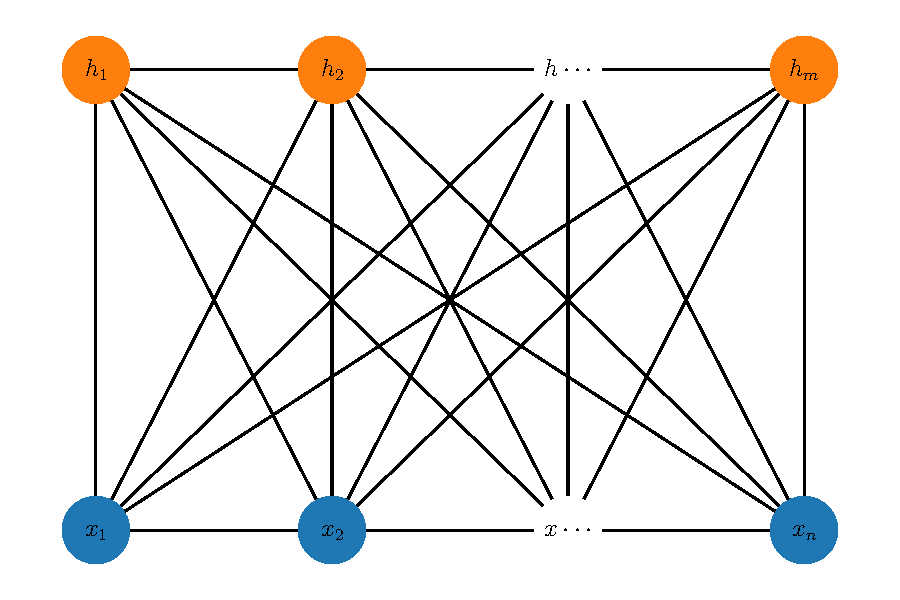
\includegraphics[scale=0.5]{latex/latex-report/Images/bm_visualize.pdf}
\end{center}
\caption{Simple visualization of a BM network with a visible layer of $n$ nodes and a hidden layer of $m$ nodes. The links between the nodes are weighted, and they are all contained within a weight matrix, $W$. The BM network is fully connected between all nodes. Every link is undirected, as the connections go both ways.}
\label{fig:vis_BM}
\end{figure}

\subsection{Restricted Boltzmann Machines}
The visible and hidden layer of the RBM is interconnected, but not intraconnected. The connections are weighted by the weight matrix $W\in\mathbb{R}^{M\times N}$


\begin{figure}[H]
\begin{center}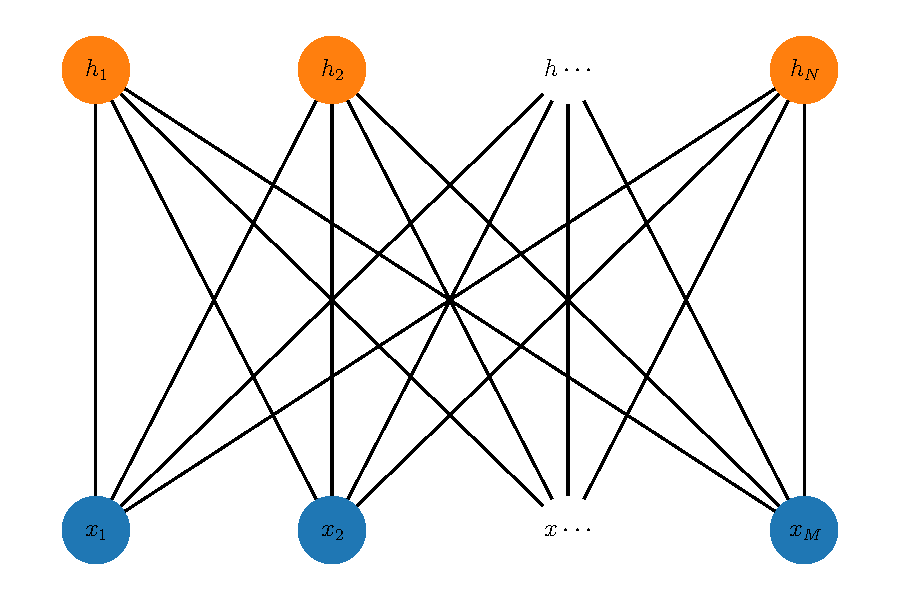
\includegraphics[scale=0.5]{latex/latex-report/Images/rbm_visualize.pdf}
\end{center}
\caption{Simple visualization of an RBM network with a visible layer of $n$ nodes and hidden layer layer of $m$ nodes. The links between the nodes are weighted, and they are all contained within a weight matrix, $W$. The RBM network is fully connected between the layers. Every link is undirected, as the connections go both ways.}
\label{fig:vis_RBM}
\end{figure}





%\newpage
%================================================================
\section{Methodology}\label{sec:Method}
%================================================================

%----------------------------------------------------------------
\subsection{Project Method 1}\label{sec:project method}
%----------------------------------------------------------------


%\newpage
%================================================================
\section{Results and Discussion}\label{sec:Results}
%================================================================

%----------------------------------------------------------------
\subsection{Non-Interacting}\label{sec:project results}
%----------------------------------------------------------------

\autoref{fig:train_iter_lr} We vary the number of training iterations and the the learning rate, $\eta$. The training, or update of parameters, are done in batches of 5000 iterations, meaning that the x-axis tick labels correspond to the number of updates. 

Each point is the average of 8 Markov chains, each with expectation value of the energy, $\langle E \rangle$, the variance $\mathrm{Var}(E)$ and sampling error, $\sigma_b$, found via the blocking method, estimated from $2^{18}$ samples. The scales of the proposal distributions, $\sigma_p$, are set to $\sigma_p=3.0$ and $\sigma_p=1.3$ for the RWM and LMH algorithms, respectively, which give acceptance rates of $\sim 30\%$ and $\sim60\%$, respectively. 

System: 1 particle in 1 dimension, 2 hidden neurons, with the variance in the Gaussian layer set as $\sigma_\mathrm{RBM}^2=1.0$

\begin{figure}[!htb]
\begin{center}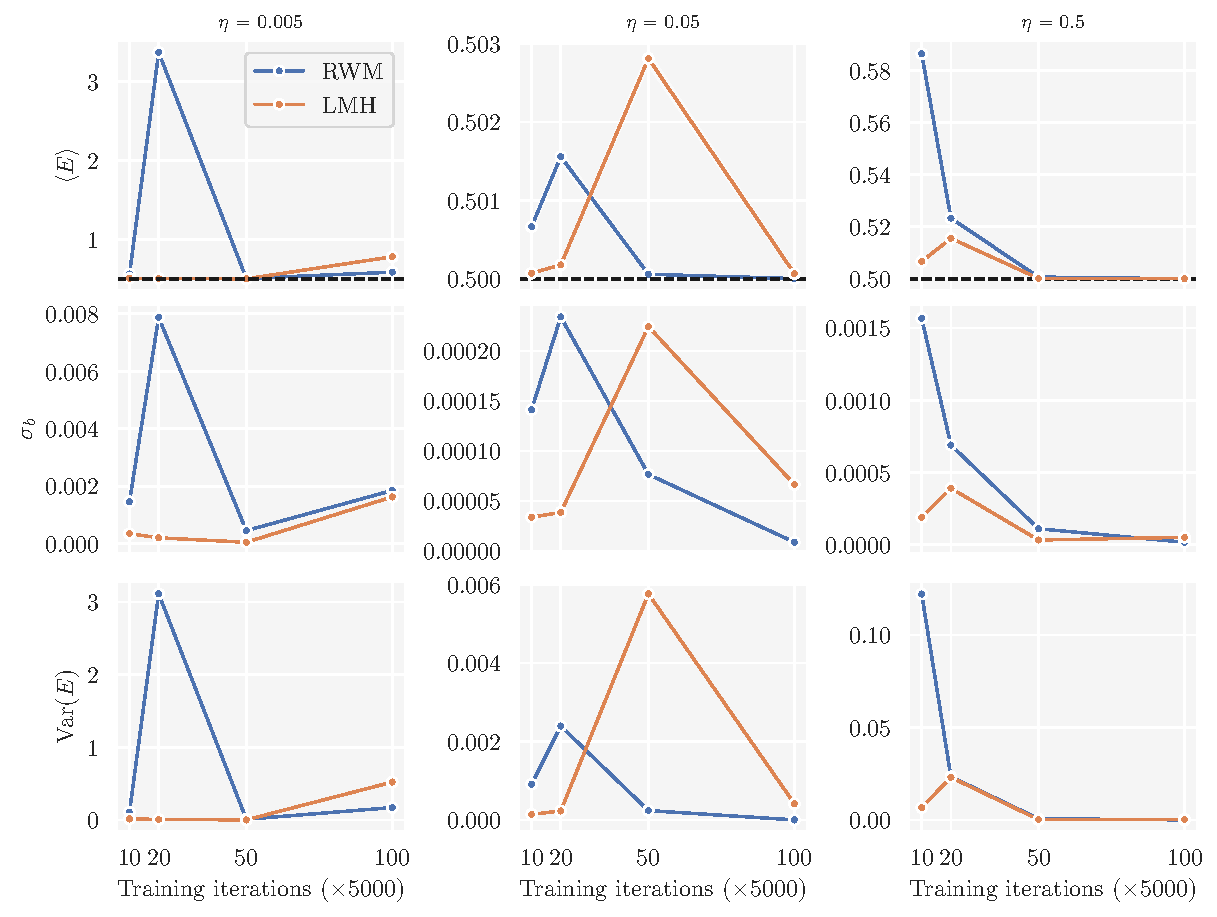
\includegraphics[width=\textwidth]{latex/figures/training_cycles_lr.pdf}
\end{center}
\caption{c}
\label{fig:train_iter_lr}
\end{figure}


%\newpage
%%================================================================
\section{Discussion}\label{sec:Discussion}
%================================================================

%----------------------------------------------------------------
\subsection{Project Discussion 1}\label{sec:project discussion}
%----------------------------------------------------------------

%================================================================
\section{Conclusion}\label{sec:Conclusion}
%================================================================

Inspired by \cite{Carleo_2017}, we have implemented a formalism using the unsupervised machine learning method \textit{restricted Boltzmann machine} (RBM) to study interacting many-particle systems. In particular, we have have used Gaussian-binary RBMs to model the wave function. In order to learn the parameters of the model, we have used a variational Monte Carlo (VMC) approach together with gradient descent optimization. For the VMC approach we consider the two Markov chain Monte Carlo (MCMC) sampling algorithms \textit{random walk Metropolis }, which is more of a brute-force sampling routine, and the \textit{Langevin Metropolis-Hastings}, which uses importance sampling. For gradient descent we have used the ADAM optimizer. We were able to accurately estimate the ground state energy for the simple system with a single one-dimensional particle, and found that, in this case, the RBM was more lenient when it came which settings produced accurate results. We found the best approximation to the ground state energy to be $E_0 = 0.499999 \pm 3\cdot10^{-6}$ a.u with ground truth $E_0=0.5$ a.u, using he RWM sampling algorithm. For the more complicated case with a couple of two-dimensional particles with repulsive interaction, finding optimal settings was more difficult. Here, we were able to obtain an energy estimate within one decimal point accuracy, $E_0 = 3.059 \pm 0.008$ a.u, of the ground truth, $E_0=3.0$ a.u, for specific settings, but others yielded estimates with significantly larger discrepancy. Our cost function is based solely on minimization of the expectation value of the energy, $\langle E \rangle$, and it might be beneficial to construct a cost function based on minimizing the variance, $\mathrm{Var}(E)$, or on minimizing both $\langle E \rangle$ and $\mathrm{Var}(E)$. 



% We consider two Markov chain Monte Carlo (MCMC) sampling algorithms; (i) the common random walk Metropolis (RWM) which explores the local neighborhood of the current state of the Markov chain using proposals from a symmetric probability distribution, and (ii) an algorithm based on the the nonlinear diffusion described by the Fokker-Planck and Langevin equations where the proposals are driven according to the gradient flow of the probability density of the trial wave function. The drift introduced in the second algorithm will typically move the Markov chain faster towards the center of the target distribution and thus mix faster than the plain RWM algorithm. We refer to the second algorithm as Langevin Metropolis-Hastings (LMH) due to its resemblance to Langevin Monte-Carlo type algorithms such as the Metropolis-adjusted Langevin algorithm (MALA) \citep{MALA}. 



% we have developed from scratch formalism and software for us- ing unsupervised machine learning methods to study interacting many-particle systems. 
%The MCMC sampling algorithms using the NQS trial wave function reached a high accuracy for the quantum dot in the single-dimensional harmonic oscillator trap, with a precision of order $10^{-6}$. The approximation to the ground state was found to be $E_0 = 0.499999 \pm 3\cdot\10^{-6}$ a.u. As for the system of two interacting electrons in the isotropic two-dimensional harmonic oscillator trap, the upper bound approximation to the ground state energy was $E_0 = 3.059\pm 0.008$ a.u. 

%Cost function - might be beneficial to use a cost function either based on minimizing the variance, Var(E), or on minimizing both $\langle E \rangle$ and Var(E). 

%The training itself is stochastic, and here we train the RBM parameters once, and then sample with the trained parameters with multiple Markov chains. A more rigorous approach would be to compare statistics across multiple training rounds with the same system and initial parameter settings

%Also train/optimize RBM scale

% The many-body wave function increases exponentially in complexity with the number of particles, and therefore, clever approximations to it is of great interest. The universal approximation theorem states that any function can be approximated to an arbitrary error by a neural network. We will therefore seek to implement an approach based on a machine learning approach. 
%An approach based on a neural network for solving the quantum mechanical wave function is still a relatively new, but an increasingly interesting prospect \citep{Saito_2018}. This paper analyzes two systems of electrons, a quantum dot in a one-dimensional harmonic oscillator trap and a pair of interacting electrons in an isotropic two-dimensional harmonic oscillator trap. We analyze the systems using an unsupervised learning method, the restricted Boltzmann machine (RBM), to simulate the wave function (known as a Neural-network Quantum State\citep{Carleo_2017}), and generate upper bound estimates to the ground state energies using two Monte Carlo approaches. We perform some coarse searches in the space of hyper parameters, like learning rate, batch-sizes for optimization and number of neurons in hidden layer. After finding the optimal set of parameters, we find that we approximate the ground state for the quantum dot in a single dimension to a high degree of precision. We find the best approximation to the ground state energy to be $E_0 = 0.499999 \pm 3\cdot10^{-6}$ a.u, using he RWM sampling algorithm. For the system of two interacting electrons in two-dimensional space we find the best approximation, again via the RWM sampling algorithm, to be $E_0 = 3.059 \pm 0.008$ a.u. Knowing the true ground state energy to be $E_0=3.0$ a.u \citep{PhysRevA.48.3561}, there is still plenty of room for improvement.

%================================================================
\section{Future Work}\label{sec:Future}
%================================================================


 
%-------- bibliography ----------- 
\newpage 
\printbibliography[heading=bibintoc, title={References}]

%-------- appendix -----------
\appendix
%================================================================
\section{Appendix}\label{sec:Appendix A}
%================================================================

 

\end{document}
%==========================================================
% ------------------- end of main content ---------------
%==========================================================
